\documentclass{beamer}
\usepackage[utf8]{inputenc}
% \usepackage[latin1]{inputenc} %  Alternativ unter Windows
% \usepackage[T1]{fontenc}
\usepackage[ngerman]{babel}
\usepackage[toc,page]{appendix}
\usepackage{latexsym}
\usepackage{amsmath,amssymb,amsthm}
\usepackage{hyperref}

\newcommand*{\quelle}{%
	\footnotesize Quelle:
}

\useoutertheme{infolines}
\beamertemplatenavigationsymbolsempty
\setbeamertemplate{headline}{}

\title{Seminar Statistische Lernverfahren}
\subtitle{Klassifikation von Rezensionstypen}
\author[T.G., M.H., A.K., M.L., T.N., J.S.]{Till Gräfenberg, Matthias Häußler, Alexander Kohlscheen, Michael Lau, Tanja Niklas, Jonathan Schmitz}
\date{12. Dezember 2019}
\begin{document}
\begin{frame}
\thispagestyle{empty}
\begin{flushright}

\includegraphics[scale=0.2]{compeon.png}
\end{flushright}
\titlepage
\end{frame}
%<-------------Folie 1--------->
\begin{frame}
\addtocounter{framenumber}{-1}
\frametitle{Inhaltsverzeichnis}
\begin{enumerate}\itemsep10pt
\item Problemstellung
\item Erstellen von Prädiktoren
\item Analysemethoden
	\begin{enumerate}
	\item Naive Bayes
	\item Entscheidungsbaum
	\item Random Forest
	\item Support Vector Machine
	\item weitere Anpassungen und Modelle
	\end{enumerate}
\end{enumerate}
\end{frame}
%<-------------Folie 1--------->
\section{Problemstellung}
\begin{frame}
\frametitle{Problemstellung}
\begin{itemize}\setlength\parskip{12pt}
\item Ziel: Klassifizierung von Reviews in folgende Typen
\begin{center}
\begin{tabular}{c|c|c}
Texttyp & introvertiert & extrovertiert \\
\hline 
emotional & stetig & initiativ\\
rational & gewissenhaft & dominant
\end{tabular}
\end{center}
\item Gegeben: 439 bereits klassifizierte Reviews
\end{itemize}
\end{frame}


%<-------------Folie 4--------->
\section{Erstellen von Prädiktoren}
\begin{frame}
\frametitle{Erstellen von Prädiktoren}
\begin{itemize}\itemsep12pt
\item Klassifikation sollte durch verwendete Wörter geschehen
\item Zurückführung auf Grundwörter notwendig
\item Benutzung verschiedener Packages in \texttt{R} bzw. \texttt{Python} ermöglichte verschiedene Verfahren.
\end{itemize}
\end{frame}

\begin{frame}
\frametitle{Erstellen von Prädiktoren}
\framesubtitle{Stemming}
\begin{itemize}\itemsep12pt
\item Durch Abschneiden von Prä-/In- und Suffixen und Ersetzen von Umlauten, Diphtongen etc. erzeugen von Wortstämmen.
\item Eigene Implementierung nach Vorgabe von COMPEON in \texttt{R}
\item Für Englische Sprache bereits vorgefertigte Tools z.B. 
\begin{itemize}
\item \texttt{porterstemmer} von \texttt{nltk} in Python
\item \texttt{snowballstemmer} von \texttt{nltk} in Python
\end{itemize}
\end{itemize}
Probleme:
\begin{itemize}
\item Unregelmäßigkeit von Verben im Deutschen
\item Komposita
\end{itemize} 
\end{frame}

\begin{frame}
\frametitle{Erstellen von Prädiktoren}
\framesubtitle{Lemmatisierung}
\begin{itemize}\itemsep12pt
\item Alternative: Zurückführung auf grammatikalische Grundformen
\item Erfordert vorgefertigte Packages z.B.
\begin{itemize}
\item \texttt{SpaCy} in Python
\item \texttt{nltk} in Python
\end{itemize}
\item Diese lieferten zusätzlich Informationen über die Wortart
\item Auch hier für Englische Sprache ausgereifter als die deutsche Alternative
\end{itemize}
\end{frame}

\begin{frame}
\frametitle{Erstellen von Prädiktoren}
\framesubtitle{Filterung der Prädikatoren, weitere}
\begin{itemize}\itemsep12pt
\item Nach Erstellung der Grundwörter konnte gefiltert werden, welche Wörter häufig auftraten
\item Denkbare Filtermethoden:
\begin{itemize}
\item Nur Wörter, die mind. $n$ Mal aufgetaucht sind 
\item Nur Wörter, die in mind. $p\%$ der Reviews verwendet wurden
\end{itemize} 
\item Anschließend Erstellung einer binären Document-Term-Matrix, die kodiert, welche Grundwörter in welchen Reviews auftauchten
\item Alternative: PCA um aussagekräftige \glqq Wörterachsen\grqq \,zu bestimmen.
\end{itemize}
\end{frame}

\begin{frame}
 \frametitle{Erstellen von Prädiktoren}
 \framesubtitle{PCA - Principal Component Analysis}
 Ziel: Dimensionsreduktion \\
 \vspace{12pt}
 Idee: Suche die Datenachsen, auf denen die Varianz am größten ist \\
 \vspace{12pt}
 Verfahren:\\
 
 \begin{itemize}
  \item Sei $X$ die DT-Matrix (Spaltenmittelwerte = 0)
  \item Bestimme die Kovarianzmatrix $Cov = X^TX$
  \item Bestimme die Eigenwerte $\lambda_i$ und Eigenvektoren $v_i$ von $Cov$
  \item Sei $V = (v_1| v_2| ...)$
  \item Transformiere die Daten zu $\hat{X} = X V$
 \end{itemize}

 \vspace{12pt}
 Problem: Die Resultate verlieren an Interpretierbarkeit
 
\end{frame}

\begin{frame}
 \frametitle{Erstellen von Prädiktoren}
 \framesubtitle{PCA - Principal Component Analysis}
 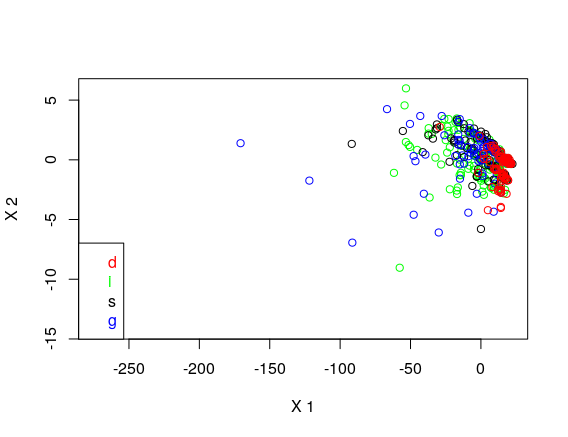
\includegraphics[scale=0.36]{PCA_1_2.png}
 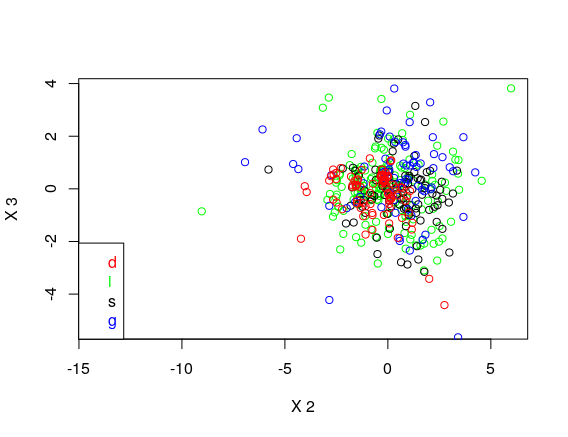
\includegraphics[scale=0.36]{PCA_2_3.png}
 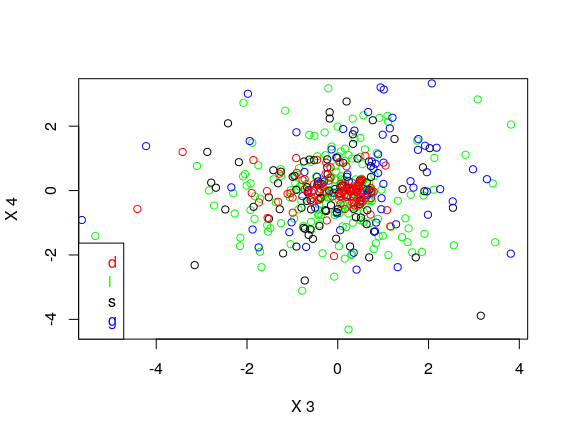
\includegraphics[scale=0.36]{PCA_3_4.png}
 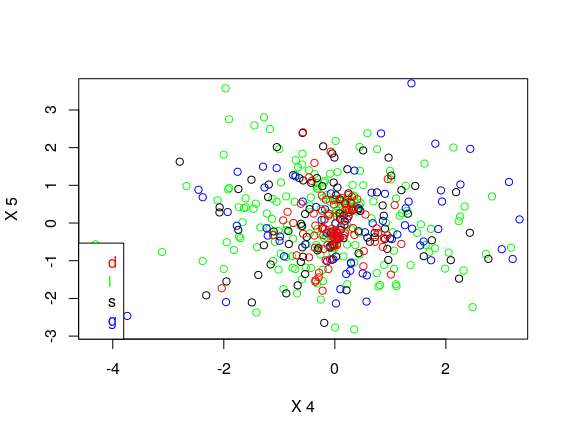
\includegraphics[scale=0.36]{PCA_4_5.png}
 
\end{frame}

\begin{frame}
 \frametitle{Erstellen von Prädiktoren}
 \framesubtitle{PCA - Principal Component Analysis}
 Fazit:
 \begin{itemize}
  \item Die Dominanten Reviews haben eine geringere Varianz
  \item keine erkennbaren Gruppen
  \item Mittelwerte der Gruppen sind ähnlich
 \end{itemize}
 
 Das Verfahren liefert keine besseren Ergebnisse. 

\end{frame}



\section{Analysemathoden}
%<-------------Folie 8--------->

% Jonathans Text
\begin{frame}
\frametitle{Analysemethoden}
\framesubtitle{Naive Bayes}
\begin{itemize}\itemsep12pt
\item Das Naive Bayes Verfahren fußt auf dem Bayes Theorem
\[p(y|x) = \frac{p(x|y)p(y)}{p(x)}\]
bzw. für unabhängige Prädiktoren $x_1,...,x_n$ als
\[p(y|x_1,...,x_n)=\frac{p(x_1|y)\cdots p(x_n|y)p(y)}{p(x_1,...,x_n)}\propto p(x_1|y)\cdots p(x_n|y)p(y).\]
\item Durch Schätzen von $p(y)$ und $p(x_i|y)$ (für die Reviewtypen $y$) durch die relativen Häufigkeiten, können wir dann Klassifikationen durchführen als
\[\hat{y}=\text{argmax}_y\,p(y)\prod_{i=1}^np(x_i|y).\]
\end{itemize}
\end{frame}

\begin{frame}
\frametitle{Analysemethoden}
\framesubtitle{Naive Bayes}
\begin{itemize}\itemsep12pt
\item Durchführung war in \texttt{R} mit dem Package \texttt{karet}, über \texttt{Python} mit \texttt{sklearn} möglich. Mit letzterem haben wir jeweils die deutschen und englischen Reviews klassifiziert.
\item Dieses Vorgehen zeigte nur wenig bessere Ergebnisse als eine einheitliche Zuweisung.
\end{itemize}
\begin{center}
(Bester) Naive Bayes, \texttt{R}, Wortaufkommen $> 20$\
\begin{tabular}{|c|c|c|c|c|c|c|c|c|}
\hline
				& D 	& G	& I & S	& Acc.	& Prec. & Recall	& F1\\
\hline
Dominant 		& 14		& 2 			& 8 		& 1 		&       	& 0,56 	& 0,778 	& 0,651\\
Gewissenhaft 	& 0 		& 0 			& 0 		& 0 		& 			& n.d. 		& 0 	& n.d.\\
Initiativ 		& 4 		& 11			& 28		& 17		& 			& 0		& 0,778 	& 0\\
Stetig 			& 0 		& 1 			& 0 		& 0 		& 			& 0	   		& 0 	& n.d\\
\hline
Total 			& 			& 				& 			& 			& 0,488		& n.d. 		& 0,389  	& n.d.\\
\hline
\end{tabular}
\end{center}
\end{frame}

\begin{frame}
\begin{center}
Naive Bayes, \texttt{Python}, Wortvorkommen in mind. 1\% der Texte,\\
Lemmatisierung mit spacy, Englisch\
\begin{tabular}{|c|c|c|c|c|c|c|c|c|}
\hline
 & D 	& G	& I & S	& Acc.	& Prec. & Recall	& F1\\
\hline
Dominant & 13 & 4 & 12 & 4 & & 0,54 & 0,722 & 0,62\\
Gewissenhaft & 0 & 3 & 3 & 0 & & 0,5 & 0,214 & 0,3\\
Initiativ & 4 & 5 & 16 & 11 & & 0 & 0,444 & 0\\
Stetig & 1 & 2 & 5 & 3 & & 0,273 & 0,167 & 0,207\\
\hline
Total  &   &   &   &   & 0,407 & 0,329  & 0,387   & 0,281\\
\hline
\end{tabular}
\end{center}
\end{frame}

\begin{frame}
\begin{center}
Naive Bayes, \texttt{Python}, Wortvorkommen in mind. 1\% der Texte,\\
Lemmatisierung mit spacy, Deutsch\
\begin{tabular}{|c|c|c|c|c|c|c|c|c|}
\hline
 & D 	& G	& I & S	& Acc.	& Prec. & Recall	& F1\\
\hline
Dominant & 16 & 2 & 13 & 2 & & 0,444 & 0,889 & 0,593\\
Gewissenhaft & 0 & 5 & 4 & 1 & & 0,5 & 0,357 & 0,417\\
Initiativ & 2 & 5 & 16 & 13& & 0 & 0,444 & 0\\
Stetig & 0 & 2 & 3 & 2& & 0,286 & 0,111 & 0,16 \\
\hline
Total  &   &   &   &   & 0,453 & 0,308  & 0,45   & 0,292\\
\hline
\end{tabular}
\end{center}
\end{frame}

\subsection{Entscheidungsbaum}
\subsection{Random Forest}
\subsection{Lineare Modelle}

\subsection{Weitere Methoden}
\begin{frame}
 \frametitle{Analysemathoden}
 \framesubtitle{weitere Anpassungen und Modelle}
 Mit Naive Bayes und den Wortarten als Prädiktoren lässt sich zuverlässig voraussagen,
 ob eine Person extrovertiert ist:\\
 \vspace{12pt}
 \begin{center}
 \begin{tabular}{r|c|c|}
  &  extrovertiert  & introvertiert \\
  \hline
  extrovertiert & 30 & 5  \\
  introvertiert & 24 & 27 \\
 \end{tabular} 
 \end{center}

 \vspace{12pt}
 
 Idee:\\
 Nutze die Vorhersage dieses Modells um ein neues Modell anzupassen.
\end{frame}

\begin{frame}
 \frametitle{Analysemathoden}
 \framesubtitle{weitere Anpassungen und Modelle}
 
 \begin{minipage}{0.45\textwidth}
  
 Random Forest\\
 \begin{center}
 \begin{tabular}{c|c|c|c|c|}
                &  D     & G  & I     & S\\
  \hline
  D      & 14            & 2             & 8             & 1 \\
  G  & 1             & 4             & 1             & 0\\
  I     & 3             & 7             & 25            & 15\\
  S        & 0             & 1             & 2             & 2
 \end{tabular}
 \end{center}
 \end{minipage}
 \begin{minipage}{0.45\textwidth}
 Random Forest mit Naive Bayes\\
 \begin{center}
  \begin{tabular}{c|c|c|c|c|}
      &  D    & G   & I     & S\\
  \hline
  D   & 15    & 2   & 9             & 1 \\
  G   & 0     & 4   & 1             & 1\\
  I   & 3     & 8   & 24            & 13\\
  S   & 0     & 0   & 2             & 3
 \end{tabular}
 \end{center}
 \end{minipage}
 
  \vspace{12pt}
 Das modifizierte Verfahren liefert im Schnitt keine besseren Ergebnisse
\end{frame}

 % Matthias Text
 \section{Analysemethoden}
\begin{frame}
\frametitle{Analysemethoden}
\framesubtitle{Entscheidungsbaum}
\begin{itemize}\setlength\parskip{12pt}
\item Teilt in Klassen auf
\item Wahr oder Falsch Entscheidungen
\item Jedes Blatt hat genau eine Klasse
\item Verwende \texttt{rpart}
\end{itemize}
\begin{center}
	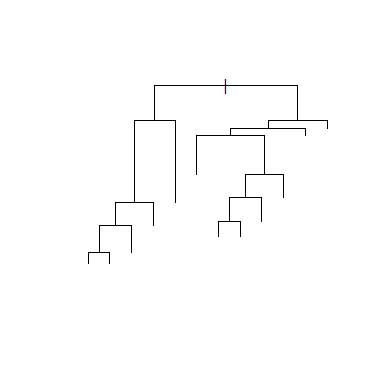
\includegraphics[scale=0.5]{RPart.png}
\end{center}
\end{frame}
%<-------------Folie--------->
\begin{frame}
\frametitle{Resultate Entscheidungsbaum, R, mind. 20 mal Wörter}
\begin{center}
\begin{tabular}{r|c|c|c|c|}
 &  Dominant  & Gewissenhaft & Initiativ & Stetig\\
\hline
Dominant & 14 & 3 & 9 & 1 \\
Gewissenhaft & 0 & 3 & 5 & 5\\
Initiativ & 2 & 4 & 19 & 5\\
Stetig & 2 & 4 & 3 & 7
\end{tabular}
\end{center}
\end{frame}
%<-------------Folie--------->
\begin{frame}
\frametitle{Resultate Entscheidungsbaum, R, mind. 20 mal Wörter}
\begin{center}
\begin{tabular}{r|c|c|c|}
 &  Precision  & Recall & F1 \\
\hline
Dominant     & 51,8\% & 77,7\% & 62,1\% \\
Gewissenhaft & 23,0\% & 21,4\% & 22,1\% \\
Initiativ    & 63,3\% & 52,7\% & 57,5\% \\
Stetig       & 43,7\% & 38,8\% & 41,1\% \\
\hline
Macro        & 45,4\% & 47,6\% & 45,4\%
\end{tabular}
\end{center}
\end{frame}
%<-------------Folie--------->
\begin{frame}
\frametitle{Resultate Entscheidungsbaum, Python, mind. in 1\% der Texte, englisch}
\begin{center}
\begin{tabular}{r|c|c|c|c|}
 &  Dominant  & Gewissenhaft & Initiativ & Stetig\\
\hline
Dominant &     9 & 4 & 12 & 5 \\
Gewissenhaft & 2 & 3 & 4 & 2\\
Initiativ &    5 & 5 & 12 & 8\\
Stetig &       2 & 2 & 8 & 3
\end{tabular}
\end{center}
\end{frame}
%<-------------Folie--------->
\begin{frame}
\frametitle{Resultate Entscheidungsbaum, Python, mind. in 1\% der Texte, englisch}
\begin{center}
\begin{tabular}{r|c|c|c|}
 &  Precision  & Recall & F1 \\
\hline
Dominant     & 30,0\% & 50,0\% & 37,5\% \\
Gewissenhaft & 27,2\% & 21,4\% & 23,9\% \\
Initiativ    & 40,0\% & 33,3\% & 36,3\% \\
Stetig       & 20,0\% & 16,6\% & 18,1\% \\
\hline
Macro        & 29,3\% & 30,3\% & 28,9\%
\end{tabular}
\end{center}
\end{frame}
%<-------------Folie--------->
\begin{frame}
\frametitle{Resultate Entscheidungsbaum, Python, mind. in 1\% der Texte, deutsch}
\begin{center}
\begin{tabular}{r|c|c|c|c|}
 &  Dominant  & Gewissenhaft & Initiativ & Stetig\\
\hline
Dominant &     13 & 4 & 16 & 1 \\
Gewissenhaft & 2 & 4 & 1 & 3\\
Initiativ &    3 & 5 & 13 & 7\\
Stetig &       0 & 1 & 6 & 7
\end{tabular}
\end{center}
\end{frame}
%<-------------Folie--------->
\begin{frame}
\frametitle{Resultate Entscheidungsbaum, Python, mind. in 1\% der Texte, deutsch}
\begin{center}
\begin{tabular}{r|c|c|c|}
 &  Precision  & Recall & F1 \\
\hline
Dominant     & 38,2\% & 72,2\% & 49,9\% \\
Gewissenhaft & 40,0\% & 28,5\% & 33,2\% \\
Initiativ    & 46,4\% & 36,1\% & 40,6\% \\
Stetig       & 50,0\% & 38,8\% & 43,6\% \\
\hline
Macro        & 43,6\% & 43,9\% & 41,8\%
\end{tabular}
\end{center}
\end{frame}
%<-------------Folie--------->
\begin{frame}
\frametitle{Analysemethoden}
\framesubtitle{Random Forest}
\begin{itemize}\setlength\parskip{12pt}
\item Entscheidungsbaum nicht beste Option
\begin{itemize}
	\item gut für Trainingsdaten
	\item nicht flexibel 
	\item Probleme mit neuen Datensätzen
\end{itemize}
\item Generiere neue Testdaten durch Wählen mit Zurücklegen
\item Erzeuge Entscheidungsbaum
\item Generiere so viele Entscheidungsbäume
\item Entscheidung durch Mehrheitsentscheidung
\item \texttt{R} \texttt{randomForest} 2000 Bäume
\end{itemize}
\end{frame}
%<-------------Folie--------->
\begin{frame}
\frametitle{Resultate Random Forest, R, mind. 20 mal Wörter}
\begin{center}
\begin{tabular}{r|c|c|c|c|}
 &  Dominant  & Gewissenhaft & Initiativ & Stetig\\
\hline
Dominant & 14 & 2 & 10& 0 \\
Gewissenhaft & 2 & 4 & 0 & 1\\
Initiativ & 2 & 7  & 25 & 14\\
Stetig & 0 & 1 & 1 &  3
\end{tabular}
\end{center}
\end{frame}
%<-------------Folie--------->
\begin{frame}
\frametitle{Resultate Random Forest, R, mind. 20 mal Wörter}
\begin{center}
\begin{tabular}{r|c|c|c|}
 &  Precision  & Recall & F1 \\
\hline
Dominant     & 53,8\% & 77,7\% & 63,5\% \\
Gewissenhaft & 57,1\% & 28,5\% & 28,0\% \\
Initiativ    & 52,0\% & 69,4\% & 59,4\% \\
Stetig       & 60,0\% & 16,6\% & 26,0\% \\
\hline
Macro        & 55,7\% & 48,0\% & 44,2\%
\end{tabular}
\end{center}
\end{frame}
%<-------------Folie--------->
\begin{frame}
\frametitle{Resultate Random Forest, Python, mind. in 1\% der Texte, englisch}
\begin{center}
\begin{tabular}{r|c|c|c|c|}
 &  Dominant  & Gewissenhaft & Initiativ & Stetig\\
\hline
Dominant & 16 & 4 & 14 & 4 \\
Gewissenhaft & 0 & 6 & 2 & 1\\
Initiativ & 1 & 4 & 16 & 9\\
Stetig & 1 & 0 & 4 & 4
\end{tabular}
\end{center}
\end{frame}
%<-------------Folie--------->
\begin{frame}
\frametitle{Resultate Random Forest, Python, mind. in 1\% der Texte, englisch}
\begin{center}
\begin{tabular}{r|c|c|c|}
 &  Precision  & Recall & F1 \\
\hline
Dominant     & 42,1\% & 88,8\% & 57,1\% \\
Gewissenhaft & 66,6\% & 42,8\% & 52,1\% \\
Initiativ    & 53,3\% & 44,4\% & 48,4\% \\
Stetig       & 44,4\% & 22,2\% & 29,6\% \\
\hline
Macro        & 51,6\% & 49,5\% & 46,8\%
\end{tabular}
\end{center}
\end{frame}
%<-------------Folie--------->
\begin{frame}
\frametitle{Resultate Random Forest, Python, mind. in 1\% der Texte, deutsch}
\begin{center}
\begin{tabular}{r|c|c|c|c|}
 &  Dominant  & Gewissenhaft & Initiativ & Stetig\\
\hline
Dominant & 15 & 4 & 15 & 2 \\
Gewissenhaft & 0 & 3 & 4 & 3\\
Initiativ & 2 & 4 & 15 & 9\\
Stetig & 1 & 3 & 2 & 4
\end{tabular}
\end{center}
\end{frame}
%<-------------Folie--------->
\begin{frame}
\frametitle{Resultate Random Forest, Python, mind. in 1\% der Texte, deutsch}
\begin{center}
\begin{tabular}{r|c|c|c|}
 &  Precision  & Recall & F1 \\
\hline
Dominant     & 41,6\% & 83,3\% & 55,4\% \\
Gewissenhaft & 30,0\% & 21,4\% & 24,9\% \\
Initiativ    & 50,0\% & 41,6\% & 45,4\% \\
Stetig       & 40,0\% & 22,2\% & 28,5\% \\
\hline
Macro        & 40,4\% & 42,1\% & 38,5\%
\end{tabular}
\end{center}
\end{frame}

% Michaels Text
\section{Analysemethoden}
\begin{frame}
\frametitle{Analysemethoden}
\framesubtitle{Support Vector Machine}
\begin{itemize}\setlength\parskip{12pt}
\item Versucht Entscheidungsgrenze (Hyperebene) zu finden, die die Distanz der nächsten Datenpunkte jeder Klasse zu ihr maximiert
\item Diese nächsten Datenpunkte sind die \textit{Support Vectors}
\end{itemize}
\begin{figure}
	\centering
	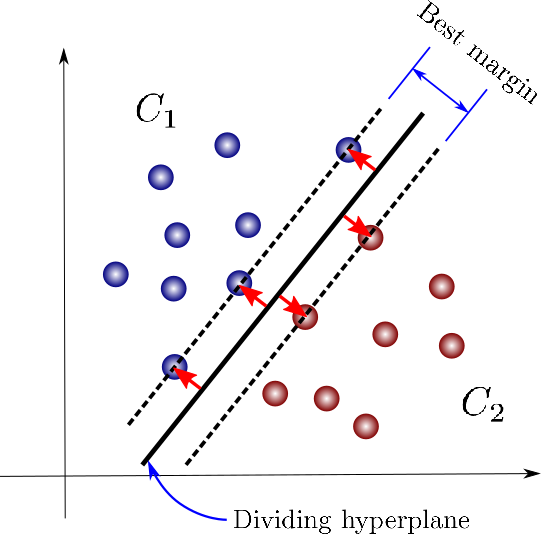
\includegraphics[scale=0.25]{svm.png}\\
	\quelle\url{https://towardsdatascience.com/support-vector-machines-for-classification-fc7c1565e3}
\end{figure}
\end{frame}
%<-------------Folie--------->
\begin{frame}
\frametitle{Analysemethoden}
\framesubtitle{Support Vector Machine}
\begin{itemize}\setlength\parskip{12pt}
	\item Verschiedene Kerne (Funktionen) um dem Separierungsproblem gerecht zu werden
	\item Kerne projizieren nicht-linear separierbare Daten niedrigerer Dimensionen auf linear-separierbare Daten höherer Dimensionen
	\item Vier häufig verwendete Kerne:
	\begin{itemize}
		\item Linear
		\item Polynomiell
		\item Radial
		\item Sigmoidal (Tangens hyperbolicus)
	\end{itemize}
	\item In \texttt{R} mit \texttt{e1071} und in Python mit \texttt{sklearn}
\end{itemize}
\end{frame}
%<-------------Folie--------->
\begin{frame}
\frametitle{Resultate Support Vector Machine, R, mind. 10 mal Wörter, Radialer Kern}
\begin{center}
\begin{tabular}{r|c|c|c|c|}
 &  Dominant  & Gewissenhaft & Initiativ & Stetig\\
\hline
Dominant & 14 & 3 & 8 & 1 \\
Gewissenhaft & 0 & 1 & 1 & 0\\
Initiativ & 4 & 10 & 27 & 14\\
Stetig & 0 & 0 & 0 & 3
\end{tabular}
\end{center}
\end{frame}
%<-------------Folie--------->
\begin{frame}
\frametitle{Resultate Support Vector Machine, R, mind. 10 mal Wörter, Radialer Kern}
\begin{center}
	\begin{tabular}{r|c|c|c|}
		& Precision  & Recall & F1 \\
		\hline
		Dominant     & 53,8\% & 77,8\% & 63,6\% \\
		Gewissenhaft & 50,0\% & 7,1\% & 16,3\% \\
		Initiativ    & 57,0\% & 75,0\% & 41,9\% \\
		Stetig       & 100,0\% & 16,7\% & 20,9\% \\
		\hline
		Macro        & 63,2\% & 44,1\% & 41,0\%
	\end{tabular}
\end{center}
Die Accuracy beträgt ca. 52,33\% und der gewichtete Macro-F1 ca. 46,2\%.
\end{frame}
%<-------------Folie--------->
\begin{frame}
\frametitle{Resultate Support Vector Machine, Python, Englisch, mind. 20 mal Wörter, Sigmoid Kern}
\begin{center}
	\begin{tabular}{r|c|c|c|c|}
		&  Dominant  & Gewissenhaft & Initiativ & Stetig\\
		\hline
		Dominant & 14 & 2 & 9 & 1 \\
		Gewissenhaft & 0 & 5 & 4 & 1\\
		Initiativ & 3 & 5 & 19 & 13\\
		Stetig & 1 & 2 & 4 & 3
	\end{tabular}
\end{center}
\end{frame}
%<-------------Folie--------->
\begin{frame}
\frametitle{Resultate Support Vector Machine, Python, Englisch, mind. 20 mal Wörter, Sigmoid Kern}
\begin{center}
\begin{tabular}{r|c|c|c|}
	& Precision  & Recall & F1 \\
	\hline
	Dominant     & 54\% & 78\% & 64\% \\
	Gewissenhaft & 50\% & 36\% & 42\% \\
	Initiativ    & 47\% & 53\% & 50\% \\
	Stetig       & 30\% & 17\% & 21\% \\
	\hline
	Macro        & 45\% & 46\% & 44\%
\end{tabular}
\end{center}
Die Accuracy beträgt ca. 47,7\% und der gewichtete Macro-F1 ca. 46\%.
\end{frame}
%<-------------Folie--------->
\begin{frame}
\frametitle{Schwierigkeiten}
\begin{itemize}
	\item Keine eindeutige Klassifikation
	\begin{itemize}
		\item Auch für Menschen nicht eindeutig
		\item Teilweise sehr geringe Unterschiede zwischen den Typen
	\end{itemize}
	\item Stemming nicht unbedingt eindeutig
	\begin{itemize}
		\item Unregelmäßigkeit von Verben im Deutschen
		\item Komposita
	\end{itemize}
	\item Geringe Zahl an Trainingsdaten
	\item Unbalanciertes Studiendesign
	\item Representativität
	\begin{itemize}
		\item Introvertierte Kunden schreiben weniger häufig Reviews
		\item Nur positive Bewertungen lagen vor
	\end{itemize}
\end{itemize}
\end{frame}






\end{document}
